\section{Konstrukcja funkcji haszujących}
\label{sec:hash_construction}
Wprawdzie konstrukcji funkcji haszujących jest wiele, większość z~nich wygląda
podobnie. Na początku skupię się na teoretycznych aspektach konstruowania
funkcji haszujących, a~w~następnej kolejności opiszę praktyczne implementacje.



\subsection{Doskonała funkcja skrótu}
W~teorii mówi się o~doskonałej funkcji skrótu, która każdy element $m$ z~danego
zbioru $M$ potrafi przekształcić w~sposób bezkolizyjny w~$h$ z~tego samego
zbioru. Innymi słowy, jest to bijekcja na samą siebie, lub permutacja.

\begin{figure}[htb!]
    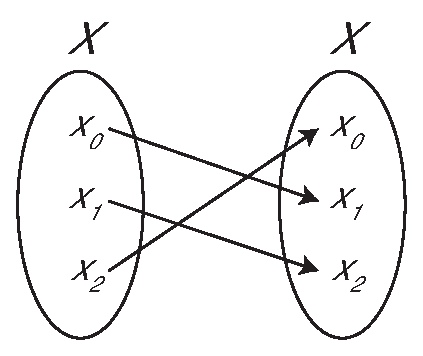
\includegraphics[width=6cm]{img/injection_self.eps}
    \caption{Każdemu wyjściu przyporządkowywane jest dokładnie jedno wejście}
    \label{fig:bijection}
\end{figure}


Znalezienie takiej funkcji w~praktyce polega na użyciu algorytmu losowego,
który dobiera każdemu $m$ przypadkowy element $h$ tak długo, aż $h$ będzie
niewykorzystany przez żaden inny element (czyli zapewniony będzie brak
kolizji):

\begin{myenumerate}

    \item Zainicjuj tablicę podstawień $T$

    \item Dla każdego $m \in M$:

    \begin{myenumerate}

        \item Wylosuj $h \in M$ takie, że $\not \exists_{m' \in M} : T_{m'} =
        h$

        \item Przydziel $T_m = h$

    \end{myenumerate}

\end{myenumerate}

Taka funkcja, mimo że na pierwszy rzut oka wydaje się przydatna
w~zastosowaniach kryptograficznych (jak by nie patrzeć, implementuje całkowicie
losowe permutacje!), jest podejściem złym z~prostych przyczyn:

\begin{itemize}

    \item Algorytm przekształcania elementów $m \in M$ na $h$ polega na
    trywialnym podstawianiu elementów zgodnie z~jakąś tablicą $T$. Zatem, aby
    uzyskać oryginalne $m$ na podstawie $h$ wystarczy odwrócić tablicę,
    zamieniając jej klucze z~przypisanymi im wartościami (dla danego $h$
    wyszukać $m$, dla którego $T_m = h$). Wykazaliśmy w~ten sposób brak
    własności \en{preimage resistance}.

    \item Gdy natomiast będziemy próbowali ukryć sposób w~jaki dokonujemy
    podstawienia (innymi słowy utajnić tablicę $T$), mamy do czynienia
    z~\en{security through obscurity} (bezpieczeństwo poprzez niezrozumiałość),
    co jest bardzo negatywnym zjawiskiem w~kryptografii i~łamie tzw. zasadę
    Kerckhoffsa. Zasada ta jest jedną z~kilku reguł sformułowanych w~XIX w.
    przez Kerckhoffsa, traktujących o~bezpieczeństwie kryptosystemów. Mówi ona,
    że każdy system kryptograficzny musi być bezpieczny nawet, gdy jego sposób
    działania wraz ze szczegółami implementacji jest jawny (za wyjątkiem
    klucza, który jest z~definicji tajny, z~tym że funkcje haszujące nie
    używają klucza).

    \item Nawet gdy zignorujemy powyższe przykazanie, nasz algorytm będzie
    nieodporny na proste ataki statystyczne: analizując rozkład
    prawdopodobieństwa pewnych wzorców wewnątrz kolejnych $h$ (który nie jest
    jednostajny, jako że w~praktyce rzadko kiedy wejście ma rozkład
    jednostajny), możemy zyskać ogólne wyobrażenie o~tym, jak wyglądają wzorce
    wewnątrz $m \in M$, co może doprowadzić do oryginalnych $m$.

    \item Wreszcie, funkcja taka jest bardzo niepraktyczna: po pierwsze, musimy
    znać z~góry \emph{wszystkie} możliwe wiadomości, jakie możemy chcieć
    zahaszować; mało tego~-- wiadomości te muszą mieć tę samą długość. Powoduje
    to, że funkcja ta nie nadaje się na kryptograficzną funkcję skrótu.

\end{itemize}



\subsection{Funkcja jednokierunkowa}
Funkcja jednokierunkowa to funkcja, której wartości dla każdego wejścia da się
łatwo obliczyć; powinno być trudne natomiast obliczenie wejścia na podstawie
posiadanego konkretnego wyjścia.

\noindent Nieformalnie, funkcja $f$ jest silnie jednokierunkowa, jeśli:

\begin{itemize}

    \item da się obliczyć w~czasie wielomianowym (czyli w~taki sposób, że czas
    działania $f$ jest w~sposób wielomianowy zależny od rozmiaru danych
    wejściowych),

    \item żaden probabilistyczny algorytm działający w~czasie wielomianowym nie
    potrafi zgadnąć argumentu z~zaniedbywalnie małym
    prawdopodobieństwem~\cite{one_way_functions}.

\end{itemize}

\noindent $f$ jest natomiast słabo jednokierunkowa, jeśli:

\begin{itemize}

    \item da się obliczyć w~czasie wielomianowym,

    \item każdy probabilistyczny algorytm działający w~czasie wielomianowym,
    który ją potrafi odwrócić, zgaduje argumenty w~sposób niepoprawny
    z~niezaniedbywalnie dużym prawdopodobieństwem~\cite{one_way_functions}.

\end{itemize}

Łatwo zauważyć, że każda silnie jednokierunkowa funkcja spełnia jednocześnie
warunki nałożone na funkcje słabo jednokierunkowe. Ponadto każda funkcja
jednokierunkowa spełnia automatycznie podstawowy warunek nałożony na bezpieczne
funkcje skrótu (mianowicie \en{preimage collision resistance}). Funkcje te
powinny zatem przyciągnąć nasze zainteresowanie.



\subsubsection{$\textrm{P} \neq \textrm{NP}$?}
Tak naprawdę nie wiadomo, czy funkcje jednokierunkowe\ldots w~ogóle istnieją.
Nie udowodniono~\cite{one_way_functions_existence} ich istnienia. Istnieją
pewne funkcje, które podejrzewamy o~jednokierunkowość, lecz nie potrafimy
wykazać poprawności lub niepoprawności tego podejrzenia.
Wykazano~\cite{one_way_functions}, że z~istnienia słabo jednokierunkowych
funkcji wynika istnienie silnie jednokierunkowych funkcji. Ponadto
udowodniono~\cite{one_way_functions}, że istnienie funkcji jednokierunkowych
implikowałoby jednocześnie, że $\textrm{P} \neq \textrm{NP}$, co dałoby
odpowiedź na jeden z~problemów milenijnych i~oznaczałoby, że klasa problemów,
które da się \emph{rozwiązać} w~czasie wielomianowym ($\textrm{P}$) nie pokrywa
się z~klasą, dla którego rozwiązanie da się \emph{zweryfikować} w~czasie
wielomianowym ($\textrm{NP}$). Przykładowo: mając liczbę $x \in \mathbb{N}$
i~dany zbiór liczb pierwszych $x_i$, możemy w~banalny sposób
\emph{zweryfikować}, czy $x_0 \cdot x_1 \cdot \ldots \cdot x_n = x$. Natomiast
nie wiadomo, czy istnieje algorytm wielomianowy, który potrafi \emph{rozwiązać}
ten problem, znajdując dla danego $x$ liczby pierwsze $x_0, x_1, \ldots, x_n$
takie, że $x_0 \cdot x_1 \cdot \ldots \cdot x_n = x$. Problem ten jest znany
jako problem rozkładu liczby na czynniki pierwsze, lub inaczej problem
faktoryzacji, i~stanowi pierwszy ze wspominanych kandydatów na funkcje
jednokierunkowe.



\subsubsection{Problem faktoryzacji}
Niech $f(S) = \prod_{s \in S} s$, gdzie $S$ jest dowolnym zbiorem liczb
pierwszych oraz $x \in \mathbb{N}$. Obliczenie $f(S)$ jest trywialne. Natomiast
obliczenie wartości odwróconej funkcji $f^{-1}(x)=S$, a~więc znalezienie dla
danej liczby $x$ jej czynników pierwszych, jest trudne, tzn. nieznany jest
żaden algorytm, który by to potrafił realizować w~czasie zależnym wielomianowo
od rozmiaru $x$~\cite{gregg2003factoring}.



\subsubsection{Problem logarytmu dyskretnego}
Niech $f(x, p, g) = g^x \mod p$, gdzie $p$ jest liczbą pierwszą, $g < p$ oraz
$x < p$. Wyliczenie tej wartości jest trywialne; nie znamy natomiast algorytmu
wielomianowego pozwalającego na zgadnięcie wartości odwróconej funkcji
\mbox{$f^{-1}(y, p, g) = x : g^x \mod p = y$} na podstawie danego $y$. Nazwa
problemu wynika z~charakteru $f$ (operacją odwrotną do potęgowania w~ciele
modulo $p$ jest logarytm w~ciele modulo $p$)~\cite{gregg2003factoring}.



\subsubsection{Funkcja Rabina}
Niech $f(x,n) = x^2 \mod n$. Wykazano, że obliczenie $f^{-1}(y,n) = x : x^2
\mod n = y$ na podstawie $y$ i~$n$ jest tak samo trudne, jak rozkład $n$ na
czynniki pierwsze; co sprowadza się do problemu faktoryzacji, opisanego
wcześniej~\cite{gregg2003factoring}.



\subsubsection{Wnioski}
Zastosowania funkcji jednokierunkowych są niejako podzbiorem tego, do czego
potrzebujemy bezpiecznych funkcji haszujących: łatwe obliczenie $f(x)$, łatwa
weryfikacja $f(x)=f(x')$ i~trudne uzyskanie odwróconej funkcji $f^{-1}(y)=x$.
Stąd też nie powinno dziwić, że ostatnim, niewymienionym dotąd kandydatem na
funkcje jednokierunkowe są\ldots kryptograficzne funkcje skrótu.

Zapotrzebowanie na funkcje jednokierunkowe jest duże, o~czym świadczy ich
wykorzystanie: trudność faktoryzacji jest zastosowana w~kryptosystemie RSA,
trudność obliczenia logarytmu dyskretnego w~podpisach cyfrowych ElGamala,
a~trudność obliczenia pierwiastka dyskretnego (funkcja Rabina)~--
w~kryptosystemie Rabina. Trudność złamania tych kryptosystemów opiera się
właśnie na trudności odwrócenia wymienionych funkcji.

Wracając na chwilę do zagadnienia $\textrm{P} \stackrel{?}{=} \textrm{NP}$~--
wystarczy udowodnić, że którakolwiek z~powyższych funkcji jest faktycznie
jednokierunkowa lub pokazać, że może zostać złamana, by móc stwierdzić to samo
o~wszystkich pozostałych wymienionych funkcjach. Jest tak dlatego, ponieważ
istnieją sposoby przekształcania jednego problemu
w~drugi~\cite{gregg2003factoring,bach1984discrete} tak, że rozwiązanie jednego
gwarantuje rozwiązanie drugiego. Zatem tak naprawdę bezpieczeństwo powyższych
kryptosystemów jest do pewnego stopnia równoważne (na tyle, na ile kosztowne są
przekształcenia problemów).



\pagebreak
\subsection{Formalnie bezpieczne funkcje skrótu}
Implementacje funkcji skrótu dzielą się na dwie kategorie. Pierwsza z~nich,
omówiona tutaj, wywodzi się z~formalnego spojrzenia na problem haszowania. Tak
naprawdę metoda ta sprowadza się do wykorzystania opisanych wcześniej
kandydatów na funkcje jednokierunkowe i~dostarczeniu dowodu, że złamanie
konstrukcji opartej na danym problemie jest tak samo trudne, jak trudne jest
rozwiązanie tego problemu. Z~charakteru tego podejścia wywodzi się nazwa tej
rodziny kryptograficznych funkcji haszujących: \en{provably secure
cryptographic hash functions}.

W~praktyce dowody trudności złamania funkcji z~tej rodziny polegają na
pokazaniu istnienia algorytmu, który przekształca w~czasie wielomianowym
problem znajdowania kolizji dla takiej funkcji w~problem rozwiązania źródłowego
problemu. W~ten sposób, kiedy zostanie znaleziony algorytm wielomianowy
potrafiący złamać formalną funkcję haszującą, będzie od razu znany sposób
szybkiego rozwiązywania problemu, na którym ta funkcja się opiera~-- a~na
chwilę obecną zakłada się, że problemy te (faktoryzacja, znajdywanie logarytmu
dyskretnego itp.) są nierozwiązywalne w~czasie wielomianowym, tak więc oznacza
to (najprawdopodobniej) sprzeczność. Możemy zatem powiedzieć, że trudność
złamania formalnych funkcji skrótu jest nie mniejsza niż trudność rozwiązania
dowolnego problemu, o~którym podejrzewamy, że jest trudny do rozwiązania.
Innymi słowy, problem złamania takich funkcji jest redukowalny do problemu
milenijnego, stąd funkcje te są postrzegane jako najbezpieczniejsze dostępne
warianty.



\subsection{Współczesne implementacje}
Wprawdzie formalnie bezpieczne funkcje skrótu są bardzo bezpieczne, nie
przychodzi to bez kosztów. Praktyka pokazuje, że funkcje te prawie w~ogóle się
nie nadają do zastosowań praktycznych lub przemysłowych z~racji swojego wolnego
działania lub wysokich kosztów pamięciowych; niestety, skutecznie eliminuje to
ich przydatność wszędzie tam, gdzie mamy do czynienia z~ograniczonymi zasobami
(przykładami mogą być: systemy wbudowane, transmisje danych w~czasie
rzeczywistym czy też systemy uwierzytelniania o~dużej przepustowości).

W~związku z~tym została stworzona druga rodzina kryptograficznych funkcji
skrótu. Działanie funkcji z~tej rodziny polega ogólnie rzecz biorąc na
dokonywaniu ogromnych liczby różnorodnych operacji na konkretnych bitach
wiadomości $m$ (takich jak przestawianie, dodawanie, odejmowanie i~inne).
Komputery są przystosowane do tego typu obliczeń, dzięki czemu w~porównaniu do
formalnie bezpiecznych funkcji skrótu haszowanie takimi funkcjami odbywa się
bardzo szybko. Oznacza to jednak, że autorzy funkcji zazwyczaj ograniczają się
jedynie do wstępnej analizy jej słabości, \latin{de~facto} nie przedstawiając
formalnego dowodu trudności jej złamania. Badania mające na celu znalezienie
słabości przypominają w~swojej naturze szukanie igły w~stogu siana:
nieznalezienie igły na daną chwilę nie oznacza jeszcze nieistnienia igły. Daje
to pole do popisu kryptologom, którzy znajdują luki na długo po pierwszym
opisaniu.



\subsubsection{Konstrukcja Merkle-Damg\r{a}rda}
Przykładem sposobu, w~jaki działają nowoczesne kryptograficzne funkcje skrótu
oparte o~operacje bitowe, może być konstrukcja Merkle-Damg\r{a}rda. Opisana po
raz pierwszy przez Merkle w~roku 1979 w~jego pracy
doktorskiej~\cite{merkle_damgard_construction}, stanowi rdzeń używanych po dziś
dzień funkcji skrótu takich jak \texttt{SHA-1} czy \texttt{MD5} i~jest jedną
z~najpopularniejszych metod konstrukcji funkcji haszujących. W~konstrukcji
wyszczególnione są abstrakcyjne elementy, które muszą być zaimplementowane
w~każdej konkretnej implementacji; spośród nich na szczególną uwagę zasługuje
funkcja dopełnienia bitowego oraz funkcja kompresji.

Nazwa wywodzi się stąd, że Merkle oraz Damg\r{a}rd, niezależnie od siebie,
udowodnili~\cite{merkle_damgard_security1,merkle_damgard_security2} w~tym samym
okresie czasu ważną własność tej konstrukcji~-- jeżeli użyty zostanie
odpowiedni schemat dopełnienia bitowego oraz zastosowana funkcja kompresji
będzie odporna na kolizje, to funkcja haszująca zbudowana za pomocą takiej
konstrukcji także będzie odporna na kolizje.

Sama konstrukcja składa się z~kroków opisanych poniżej.

\begin{myenumerate}

    \item Niech $M = \mathtt{Pad}(m)$, gdzie $m$ to wiadomość, a~$\mathtt{Pad}$
    to funkcja dopełnienia bitowego. Zadaniem tej funkcji jest przekształcenie
    wiadomości $m$ o~dowolnej liczbie bitów na wiadomość $M$ o~liczbie bitów
    podzielnej przez z~góry określoną wartość $c$. Trywialnym przykładem
    funkcji dopełnienia bitowego może być funkcja, która dopisuje z~prawej
    strony wiadomości $m$ pojedynczy bit 1, a~po nim $n$ bitów 0; dodatkowo
    często dopisywana jest długość oryginalnej wiadomości $m$.

    \item Podziel $M$ na $n$ bloków, każdy o~stałej długości $c$, niezależnej
    od $m$. Robimy to, ponieważ funkcja kompresji, opisana w~następnych
    krokach, z~definicji może działać jedynie na blokach o~stałej długości $c$.

    \item Niech $h = \mathtt{IV}$, gdzie $\mathtt{IV}$ jest z~góry określonym
    wektorem początkowym (\en{initialization vector}), zawierającym jakaś stałą
    wartość. $h$ będzie się zmieniało podczas działania konstrukcji i~oznaczać
    będzie aktualnie obliczoną wartość skrótu. Długość $h$ jest przez cały czas
    stała.

    \item Dla $i = 0, 1, \ldots, n$:

    \begin{myenumerate}

        \item Niech $h=\mathtt{Comp}(h,M_i)$, gdzie $\mathtt{Comp}$ jest
        funkcją kompresji, $h$ aktualnie obliczoną wartość skrótu a~$M_i$
        stanowi $i$-ty blok wiadomości $M$.

    \end{myenumerate}

    \item Niech $h=\mathtt{Fin}(h)$ gdzie $\mathtt{Fin}$ jest funkcją
    finalizującą. Jest to opcjonalny krok, który ma zagwarantować dodatkowe
    bezpieczeństwo poprzez np. zapewnienie lepszego efektu lawinowego.

\end{myenumerate}

\begin{figure}[H]
    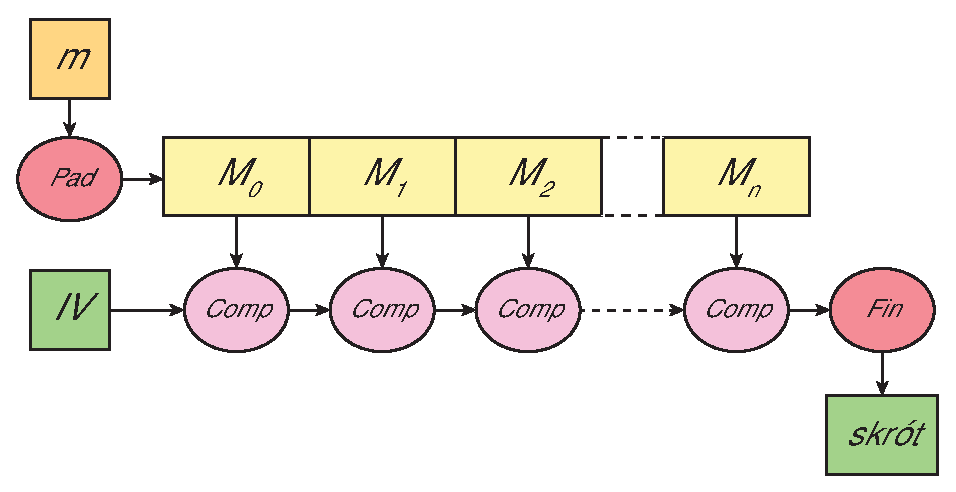
\includegraphics[width=12cm]{img/merkle_damgard.eps}
    \caption{Schemat działania konstrukcji Merkle-Damg\r{a}rda. Oznaczenia:
    $m$~-- wiadomość wejściowa, $\mathtt{Pad}$~-- funkcja dopełnienia bitowego,
    $M_0, M_1, M_2, \ldots, M_n$~-- kolejne bloki wiadomości długości $c$,
    $\mathtt{IV}$~-- wektor początkowy, $\mathtt{Comp}$~-- funkcja kompresji,
    $\mathtt{Fin}$~-- funkcja finalizująca.}
    \label{fig:merkle_damgard}
\end{figure}



\subsubsection{\texttt{MD5}}
\texttt{MD5} jest pierwszą z~dwóch funkcji, na których się skupimy w~tej pracy.
Jej wykorzystanie jest bardzo szerokie: znajduje zastosowanie w~systemach
bezpieczeństwa oraz systemach weryfikacji integralności danych (pomimo faktu,
że już w~latach 90-tych wyraźnie odradzano jej wykorzystania z~powodu
poważnych wątpliwości co do jej faktycznego bezpieczeństwa, które z~czasem
okazały się uzasadnione~\cite{ps3_attack}).

Oparta o~konstrukcję Merkle-Damg\r{a}rda, funkcja przekształca wiadomości
o~dowolnej liczbie bitów na skróty o~stałej długości 128~bitów. Jej
schemat~\cite{md5_definition} został przedstawiony poniżej (wszystkie operacje
są dokonywane w~porządku bitowym \en{little endian}; znaczenie tego terminu
oraz operatorów wprowadzonych w~tej sekcji zostało opisane
w~dodatku~\ref{app:bitwise_operations}).

\begin{myenumerate}

    \item Faza dopełnienia bitowego

    \begin{myenumerate}

        \item Dopisz bit $1$ na końcu wiadomości $m$.

        \item Dopisz tyle bitów $0$ na końcu wiadomości $m$, ile potrzeba, aby
        długość $m$ była mniejsza o~64~bity od wielokrotności 512. Innymi
        słowy, dopisz $512 \cdot \ceil{\frac{|m|+64}{512}}-64-(|m| \mod{512})$
        bitów $0$, gdzie $|m|$ oznacza długość wiadomości $m$.
        \footnote{Dopełniamy wiadomość $m$ w~taki skomplikowany sposób dlatego,
        że za chwilę będziemy dopisywać do niej nową wartość $x$ (o~długości
        64~bitów). Gdybyśmy po prostu zawinęli $m$ do 512~bitów, a~następnie
        nadpisali ostatnie 64~bity bitami $x$, mogłoby się zdarzyć, że
        nadpisalibyśmy bity oryginalnej $m$, co jest niepożądane~-- dlatego
        dbamy, aby długość wiadomości \emph{po dopisaniu} była podzielna przez
        512.}

        \item Dopisz na końcu wiadomości zakodowaną długość oryginalnej
        wiadomości $m$ (wpisując tam kolejne bity $|m| \mod{2^{64}}$).

        Ma to na celu zapewnienie własności sformułowanych przez Mihira
        Bellare, który pokazał~\cite{merkle_damgard_strengthening}, że aby
        konstrukcja Merkle-Damg\r{a}rda była bezpieczna, wystarcza, by funkcja
        $\mathtt{Pad}$ spełniała następujące własności:

        \begin{itemize}

            \item $m$ jest prefiksem $\mathtt{Pad}(m)$,

            \item gdy $|m_1| = |m_2|$, to $|\mathtt{Pad}(m_1)| =
            |\mathtt{Pad}(m_2)|$,

            \item gdy $|m_1| \neq |m_2|$, to $\mathtt{Pad}(m_1)_n \neq
            \mathtt{Pad}(m_2)_n$, gdzie $X_n$ to ostatni blok $X$. (Długość
            bloku w~tym kontekście jest taka sama, jak długość bloku używanego
            przez całą konstrukcję Merkle-Damg\r{a}rda.)

        \end{itemize}

    \end{myenumerate}

    \item Faza kompresji

    \begin{myenumerate}

        \item Na początku zostaje wprowadzony wewnętrzny stan funkcji skrótu,
        będący wektorem 128~bitów, w~którym wyróżniamy 4~wektory oznaczone
        kolejno: $A$, $B$, $C$~i~$D$ (każdy o~długości 32~bitów). Wektor ten
        jest inicjowany stałym wektorem $\mathtt{IV}$ zgodnym z~poniższym
        równaniem:

        \[
            \begin{aligned}
                A &:= \mathtt{0x67452301} \\
                B &:= \mathtt{0xefcdab89} \\
                C &:= \mathtt{0x98badcfe} \\
                D &:= \mathtt{0x10325476}
            \end{aligned}
        \]

        \item Następnie dla każdego kolejnego 512-bitowego bloku wiadomości
        \break $M_0, M_1, M_2, \ldots, M_n$ będziemy aktualizować stan
        wewnętrzny $(A,B,C,D)$ wartością funkcji kompresji obliczoną na
        podstawie poprzedniej jego wartości oraz danego bloku wiadomości $M_k$.
        Funkcja kompresji przebiega w~następujący sposób:

        \begin{itemize}

            \item Podziel blok wiadomości $M_k$ na $16$ fragmentów $W_{0 \leq j
            \leq 15}$, każdy o~długości 32~bitów.

            \pagebreak
            \item Wykonaj 4~rundy:

            \begin{itemize}

                \item Wybierz funkcję rundy~$F$ zgodnie
                z~tabelą~\ref{tbl:md5_round_function}.

                \item Wykonaj 16~operacji przekształcających stan $(A,B,C,D)$
                na podstawie jego poprzedniej wartości, funkcji rundy~$F$ oraz
                wektorów~$W$. Konstrukcja pojedynczej operacji została
                przedstawiona na rysunku~\ref{fig:md5_operation}.

            \end{itemize}

        \end{itemize}

    \end{myenumerate}

    \item Po wykonaniu wszystkich 64~operacji (4~rundy $\times$ 16~operacji),
    stan wewnętrzny $(A,B,C,D)$ jest zwracany jako wyjściowy skrót z~funkcji.

\end{myenumerate}

\begin{table}[htb]
    \caption{Funkcja $F$ użyta w~kolejnych rundach \texttt{MD5}.}
    \label{tbl:md5_round_function}
    \begin{tabular}{|l|l|}
        \hline
        Runda & Funkcja rundy \\
        \hline
        Runda 1 &
        $F(B,C,D) = (B \land C) \lor (\lnot B \land D)$ \\

        Runda 2 &
        $F(B,C,D) = (B \land D) \lor (C \land \lnot D)$ \\

        Runda 3 &
        $F(B,C,D) = B \oplus C \oplus D$ \\

        Runda 4 &
        $F(B,C,D) = C \oplus (B \lor \lnot D)$ \\
        \hline
    \end{tabular}
\end{table}

\begin{table}[htb]
    \resizebox{\columnwidth}{!}{
    \begin{tabular}{ |c|c|c|| c|c|c|| c|c|c|| c|c|c| }
        \hline
            \multicolumn{3}{|c||}{Runda 1} &
            \multicolumn{3}{|c||}{Runda 2} &
            \multicolumn{3}{|c||}{Runda 3} &
            \multicolumn{3}{|c|}{Runda 4} \\
        \hline
        $i$ & $K_i$ & $S_i$ & $i$ & $K_i$ & $S_i$ & $i$ & $K_i$ & $S_i$ & $i$ & $K_i$ & $S_i$ \\
        \hline
        0 & $\mathtt{0xd76aa478}$ & 7 & 16 & $\mathtt{0xf61e2562}$ & 5 & 32 & $\mathtt{0xfffa3942}$ & 4 & 48 & $\mathtt{0xf4292244}$ & 6 \\
        1 & $\mathtt{0xe8c7b756}$ & 12 & 17 & $\mathtt{0xc040b340}$ & 9 & 33 & $\mathtt{0x8771f681}$ & 11 & 49 & $\mathtt{0x432aff97}$ & 10 \\
        2 & $\mathtt{0x242070db}$ & 17 & 18 & $\mathtt{0x265e5a51}$ & 14 & 34 & $\mathtt{0x6d9d6122}$ & 16 & 50 & $\mathtt{0xab9423a7}$ & 15 \\
        3 & $\mathtt{0xc1bdceee}$ & 22 & 19 & $\mathtt{0xe9b6c7aa}$ & 20 & 35 & $\mathtt{0xfde5380c}$ & 23 & 51 & $\mathtt{0xfc93a039}$ & 21 \\
        4 & $\mathtt{0xf57c0faf}$ & 7 & 20 & $\mathtt{0xd62f105d}$ & 5 & 36 & $\mathtt{0xa4beea44}$ & 4 & 52 & $\mathtt{0x655b59c3}$ & 6 \\
        5 & $\mathtt{0x4787c62a}$ & 12 & 21 & $\mathtt{0x02441453}$ & 9 & 37 & $\mathtt{0x4bdecfa9}$ & 11 & 53 & $\mathtt{0x8f0ccc92}$ & 10 \\
        6 & $\mathtt{0xa8304613}$ & 17 & 22 & $\mathtt{0xd8a1e681}$ & 14 & 38 & $\mathtt{0xf6bb4b60}$ & 16 & 54 & $\mathtt{0xffeff47d}$ & 15 \\
        7 & $\mathtt{0xfd469501}$ & 22 & 23 & $\mathtt{0xe7d3fbc8}$ & 20 & 39 & $\mathtt{0xbebfbc70}$ & 23 & 55 & $\mathtt{0x85845dd1}$ & 21 \\
        8 & $\mathtt{0x698098d8}$ & 7 & 24 & $\mathtt{0x21e1cde6}$ & 5 & 40 & $\mathtt{0x289b7ec6}$ & 4 & 56 & $\mathtt{0x6fa87e4f}$ & 6 \\
        9 & $\mathtt{0x8b44f7af}$ & 12 & 25 & $\mathtt{0xc33707d6}$ & 9 & 41 & $\mathtt{0xeaa127fa}$ & 11 & 57 & $\mathtt{0xfe2ce6e0}$ & 10 \\
        10 & $\mathtt{0xffff5bb1}$ & 17 & 26 & $\mathtt{0xf4d50d87}$ & 14 & 42 & $\mathtt{0xd4ef3085}$ & 16 & 58 & $\mathtt{0xa3014314}$ & 15 \\
        11 & $\mathtt{0x895cd7be}$ & 22 & 27 & $\mathtt{0x455a14ed}$ & 20 & 43 & $\mathtt{0x04881d05}$ & 23 & 59 & $\mathtt{0x4e0811a1}$ & 21 \\
        12 & $\mathtt{0x6b901122}$ & 7 & 28 & $\mathtt{0xa9e3e905}$ & 5 & 44 & $\mathtt{0xd9d4d039}$ & 4 & 60 & $\mathtt{0xf7537e82}$ & 6 \\
        13 & $\mathtt{0xfd987193}$ & 12 & 29 & $\mathtt{0xfcefa3f8}$ & 9 & 45 & $\mathtt{0xe6db99e5}$ & 11 & 61 & $\mathtt{0xbd3af235}$ & 10 \\
        14 & $\mathtt{0xa679438e}$ & 17 & 30 & $\mathtt{0x676f02d9}$ & 14 & 46 & $\mathtt{0x1fa27cf8}$ & 16 & 62 & $\mathtt{0x2ad7d2bb}$ & 15 \\
        15 & $\mathtt{0x49b40821}$ & 22 & 31 & $\mathtt{0x8d2a4c8a}$ & 20 & 47 & $\mathtt{0xc4ac5665}$ & 23 & 63 & $\mathtt{0xeb86d391}$ & 21 \\
        \hline
    \end{tabular}
    }
    \caption{Stałe $K_i$ oraz $S_i$ użyte w~kolejnych operacjach
    podczas działania funkcji kompresji \texttt{MD5}.}
    \label{tbl:md5_operation_const}
\end{table}

\begin{figure}[H]
    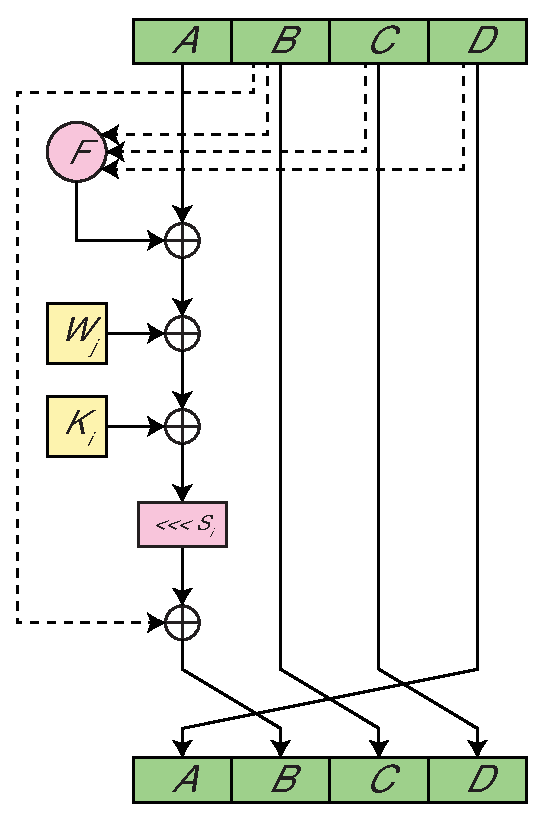
\includegraphics[width=7.5cm]{img/md5_operation.eps}
    \captionsetup{singlelinecheck=off}
    \caption[blablabla]{
    Jedna operacja \texttt{MD5}. Oznaczenia:
    \begin{itemize}
        \item $A$, $B$, $C$~i~$D$~-- wektory stanu wewnętrznego,
        \item $F$~-- funkcja rundy,
        \item $W_j$~-- $j$-ty 32-bitowy fragment pochodzący od 512-bitowego
        bloku wiadomości,
        \item $K_i$~-- 32-bitowa stała,
        \item $S_i$~-- stała oznaczająca ilość bitów w~przesunięciu cyklicznym,
        \item $i$~-- numer operacji w~kontekście funkcji kompresji ($i \in (0,
        1, \ldots, 63)$),
        \item $j$~-- numer operacji w~danej rundzie ($j \in (0, 1, \ldots,
        15)$).
    \end{itemize}
    Każda kolejna operacja używa innego zestawu stałych $K_i$ oraz $S_i$, które
    zostały opisane w~tabeli~\ref{tbl:md5_operation_const}.}
    \label{fig:md5_operation}
\end{figure}



\pagebreak
\subsubsection{\texttt{SHA-1}}
Funkcja \texttt{SHA-1}, podobnie jak funkcja \texttt{MD5}, oparta jest
o~konstrukcję Merkle-Damg\r{a}rda. Została skonstruowana przez \enn{National
Security Agency}; jej nazwa wywodzi się od \en{Secure Hash Algorithm}
(bezpieczna funkcja haszująca). \texttt{SHA-1} jest jedną z~serii funkcji
\texttt{SHA} i~choć po niej przyszły kolejne, bezpieczniejsze funkcje, to
w~obecnej chwili jest najpopularniejszą funkcją z~serii \texttt{SHA}.
\texttt{SHA-1} zwraca skróty o~długości 160~bitów. Konstrukcja
funkcji~\cite{sha1_definition} została przedstawiona poniżej.

\begin{myenumerate}

    \item Faza dopełnienia bitowego: wygląda tak samo, jak faza dopełnienia
    bitowego funkcji \texttt{MD5}.

    \item Faza kompresji

    \begin{myenumerate}

        \item Wprowadzamy wewnętrzny stan, będący wektorem 160~bitów, w~którym
        wyróżniamy 5~wektorów oznaczonych kolejno: $A$, $B$, $C$, $D$ i~$E$
        (każdy o~długości 32~bitów). Wektor ten jest inicjowany wartościami na
        podstawie stałego wektora $\mathtt{IV}$:

        \[
            \begin{aligned}
                A &:= \mathtt{0x67452301} \\
                B &:= \mathtt{0xefcdab89} \\
                C &:= \mathtt{0x98badcfe} \\
                D &:= \mathtt{0x10325476} \\
                E &:= \mathtt{0xc3d2e1f0}
            \end{aligned}
        \]

        \item Dla każdego kolejnego 512-bitowego bloku wiadomości \break $M_0,
        M_1, M_2, \ldots, M_n$ aktualizujemy stan wewnętrzny funkcją kompresji,
        która przebiega w~następujący sposób:

        \begin{itemize}

            \item Podziel blok wiadomości $M_k$ na $16$ fragmentów $W_{0 \leq i
            \leq 15}$, każdy o~długości 32~bitów.

            \item Skonstruuj dodatkowe wektory $W_{16 \leq i \leq 79}$ zgodnie
            z~wzorem:

            $$
                W_i = (W_{i-3} \oplus W_{i-8} \oplus W_{i-14} \oplus W_{i-16})
                \llless 1
            $$

            \item Wykonaj 4~rundy:

            \begin{itemize}

                \item Wybierz funkcję rundy~$F$ oraz stałą rundy~$K$ zgodnie
                z~tabelą~\ref{tbl:sha1_round_function}.

                \item Wykonaj 20~operacji przekształcających stan $(A,B,C,D,E)$
                na podstawie jego poprzedniej wartości, funkcji rundy~$F$,
                stałej rundy~$K$ oraz wektorów~$W$. Konstrukcja pojedynczej
                operacji została przedstawiona na
                rysunku~\ref{fig:sha1_operation}.

            \end{itemize}

        \end{itemize}

    \end{myenumerate}

    \item Po wykonaniu wszystkich 80~operacji (4~rundy $\times$ 20~operacji),
    stan wewnętrzny $(A,B,C,D,E)$ jest zwracany jako wyjściowy skrót z~funkcji.

\end{myenumerate}

\begin{table}[H]
    \caption{Funkcja $F$ oraz stała $K$ użyta w~kolejnych rundach
    \texttt{SHA-1}.}
    \label{tbl:sha1_round_function}
    \begin{tabular}{|l|l|l|}
        \hline
        Runda & Funkcja rundy & Stała K \\
        \hline
        Runda 1 &
        $F(B,C,D) = (B \land C) \lor (\lnot B \land D)$ &
        $K = \mathtt{0x5a827999}$ \\

        Runda 2 &
        $F(B,C,D) = B \oplus C \oplus D$ &
        $K = \mathtt{0x6ed9eba1}$ \\

        Runda 3 &
        $F(B,C,D) = (B \land C) \lor (B \land D) \lor (C \land D)$ &
        $K = \mathtt{0x8f1bbcdc}$ \\

        Runda 4 &
        $F(B,C,D) = B \oplus C \oplus D$ &
        $K = \mathtt{0xca62c1d6}$ \\
        \hline
    \end{tabular}
\end{table}

\begin{figure}[H]
    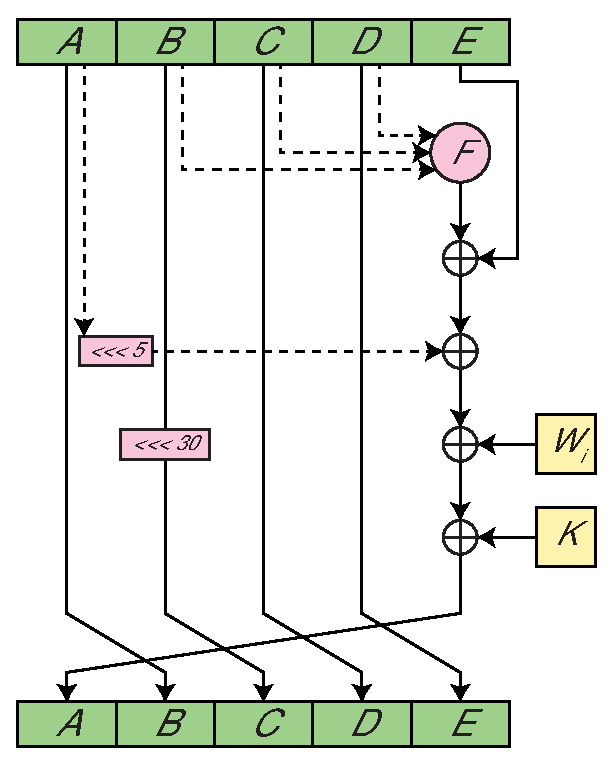
\includegraphics[width=8.5cm]{img/sha1_operation.eps}
    \captionsetup{singlelinecheck=off}
    \caption[blablabla]{
    Jedna operacja \texttt{SHA-1}. Oznaczenia:
    \begin{itemize}
        \item $A$, $B$, $C$, $D$~i~$E$~-- wektory stanu wewnętrznego,
        \item $F$~-- funkcja rundy,
        \item $K$~-- 32-bitowa stała rundy,
        \item $W_i$~-- $i$-ty 32-bitowy fragment pochodzący od rozszerzenia
        512-bitowego bloku wiadomości,
        \item $i$~-- numer operacji w~kontekście funkcji kompresji ($i \in (0,
        1, \ldots, 79)$).
    \end{itemize}}
    \label{fig:sha1_operation}
\end{figure}
